
\hypertarget{Analyse-et-traitement-des-donnuxe9es}
\section{Les signaux}
\label{Les-signaux}}

Afin d'améliorer la lisibilité des chapitres suivants nous prendrons 3 signaux (le n°17000 et le n°20000 de la base labelisée ainsi que le n°571 de la base non labelisée) que nous observerons sous diverses formes puis sur lesquels nous effectuerons un certain nombre de traitements.

\hypertarget{Signaux-Bruts}{%}
\subsection{Les signaux bruts}
\label{Signaux-Bruts}}

Dans un premier temps on commence par observer les signaux sans traitement sous différentes formes. Ces signaux sont spécifiquements choisis car ils représentent approximativement la variété des signaux que l'on a dans notre base à savoir :
\begin{itemize}
\item Des signaux très propres
\item Des signaux un peux bruités ou altérés
\item Des signaux très dégradés
\end{itemize}

\begin{figure}[!h]
\centering
	\begin{subfigure}[b]{0.3\textwidth}
    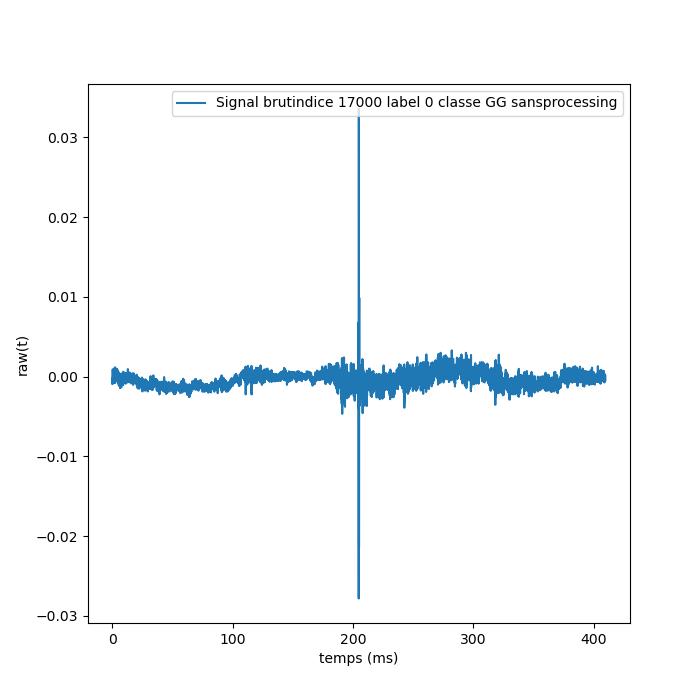
\includegraphics[width=\textwidth]{./images/indice17000Spectro1Dlabel0classeGGsansprocessingsanszoom.png}
    \caption{}
  	\end{subfigure}
  	\begin{subfigure}[b]{0.3\textwidth}
    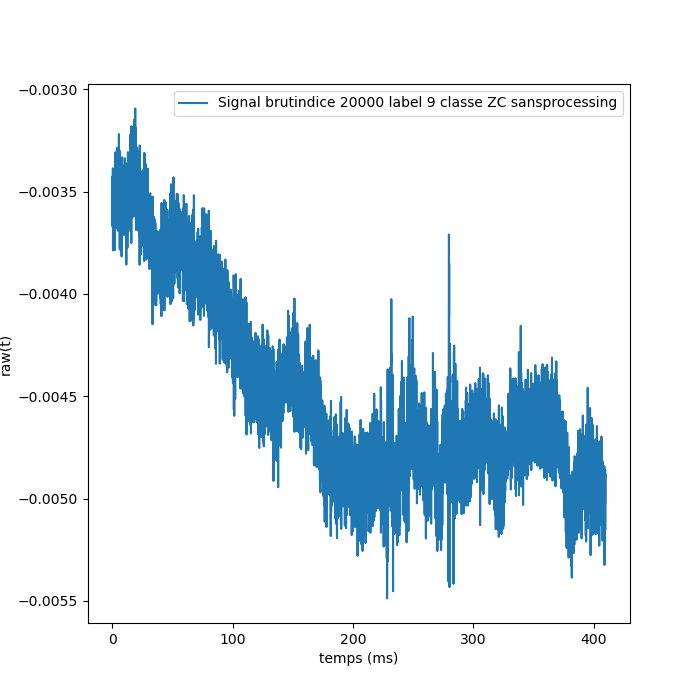
\includegraphics[width=\textwidth]{./images/indice20000Spectro1Dlabel9classeZCsansprocessingsanszoom.png}
	\caption{}
  	\end{subfigure}
  	\begin{subfigure}[b]{0.3\textwidth}
    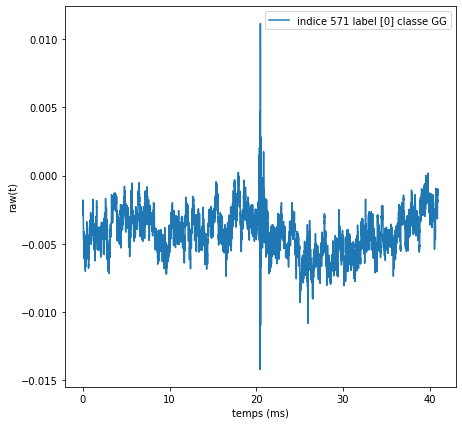
\includegraphics[width=\textwidth]{./images/indice571Spectro1Dlabel9classeZCsansprocessingsanszoom.png}
    	\caption{}
	\end{subfigure}
\caption{Signaux bruts : (a) n°17000 et (b) n°20000 de la base d'apprentissage ; (c) n°571 de la base de test.%
\label{fig:signauxbruts}}
\end{figure}

Sur la figure \ref{fig:signauxbruts}, nous constatons plusieurs choses : tout d'abord il semble y avoir une certaine disparité entre les signaux, certains étant beaucoup plus bruités que d'autres ; de plus contrairement à ce que l'on pouvait penser, le clic n'est pas toujours facile à distinguer et celui ci n'est pas non plus toujours bien centré.

Cependant nous avons pu tirer quelques enseignements de l'observation de ces signaux :
\begin{itemize}
\item L'amplitude des clics semble variable.
\item Il arrive que le bruit soit parfois suffisament important par rapport au clic pour rendre son identification difficile voir impossible.
\end{itemize}

Pour afiner notre analyse, il parait pertinent de commencer par zoomer sur ce clic.
Pour cela il va donc faloir commencer par trouver un moyen d'isoler le clic.

\hypertarget{Le-zoom}{%}
\subsection{Le zoom}
\label{Le-zoom}}

Pour zoomer sur le clic on identifie le maximum qui sera logiquement le milieu du clic puis on rajoute l'équivalent de la durée d'un clic (que nous avons obtenus grâce a une procédure préalable) avant et aprés ce maximum.


\begin{figure}[!h]
  \centering
  \begin{subfigure}[b]{0.3\textwidth}
    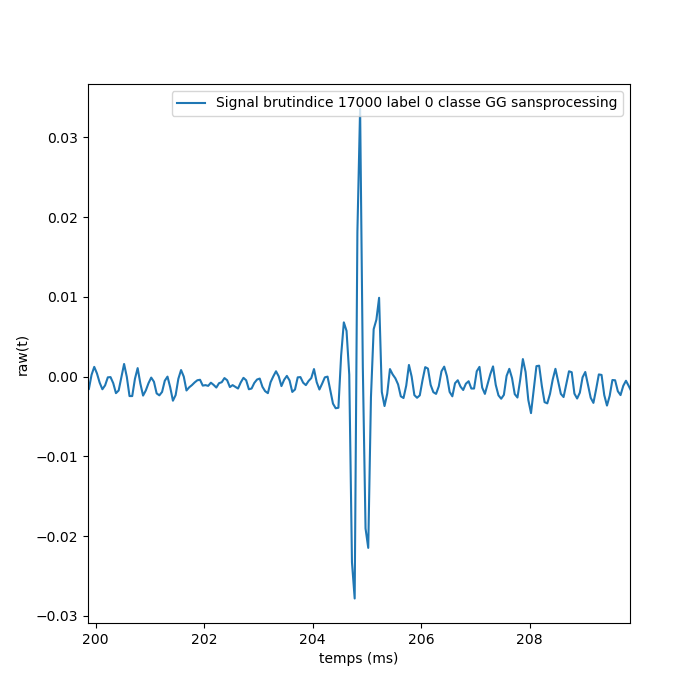
\includegraphics[width=\textwidth]{./images/indice17000Spectro1Dlabel0classeGGsansprocessingaveczoom.png}
    \caption{17000}
  \end{subfigure}
  \begin{subfigure}[b]{0.3\textwidth}
    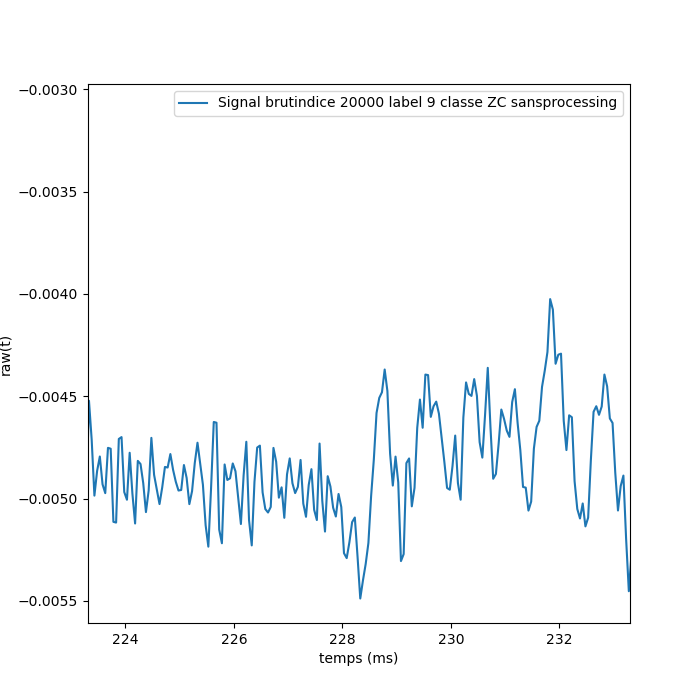
\includegraphics[width=\textwidth]{./images/indice20000Spectro1Dlabel9classeZCsansprocessingaveczoom.png}
  \caption{20000}
  \end{subfigure}
  \begin{subfigure}[b]{0.3\textwidth}
    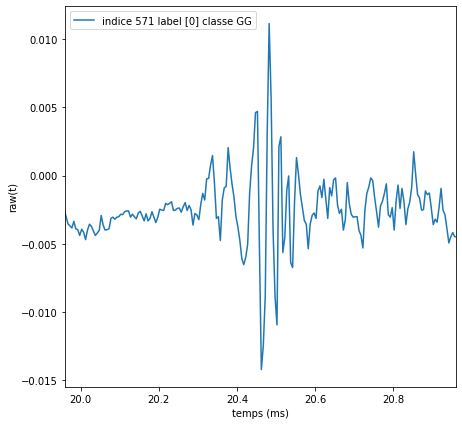
\includegraphics[width=\textwidth]{./images/indice571Spectro1Dlabel9classeZCsansprocessingaveczoom.png}
  \caption{571}
  \end{subfigure}
  \caption{Signaux bruts : (a) n°17000 et (b) n°20000 de la base d'apprentissage ; (c) n°571 de la base de test. avec un zoom temporel%
  \label{fig:signauxbrutszoom}}
\end{figure}

Or on constate que celà ne suffit pas dans tous les cas en effet si pour les signaux n° 17 000 et 571 le zoom semble bien fonctionner dans le cas du signal n° 20 000 qui est très bruité le bruit semble avoir pris le dessus sur le clic conduisant à l'echec de l'identification du clic.
On vas donc par la suite appliquer un filtre pour supprimer les bruits parasites (dont on reparlera dans la partie traitement du signal).

On peux déjà observer plusieurs phénoménes :
-tout d'abord l'efficacité du zoom semble corélée à la qualité du signal de départ
-Les "bons clics" semblent se situer aux alentours de 200 ms (ils sont donc bien centrés)
-Leur intensité est très  variable pouvant aller jusqu'a un facteur 10 entre 2 clics. Il parait donc pertinent par la suite de les normaliser.
-Leur durée est bien d'environs 5 millisecondes
Sous cette forme, nos observations semblent quand même limitées. On va donc commencer par les observer sous d'autres formes puis on cherchera à améliorer la qualité de nos signaux via diverses techniques. Etant donné la nature de nos données à savoir des enregistrements audios observer leurs spectrogrammes semble être pertinent.

\hypertarget{Transformuxe9-de-Fourier}{%}
\subsection{Transformée de Fourier}
\label{Transformuxe9-de-Fourier}}

Avant d'observer les spectrogrammes il convient de commencer par expliquer et observer les Transformés de Fourier de nos 3 signaux.

La Transformés de Fourier est un outil mathématique nous permettant de passer du domaine temporel au domaine fréquenciel.

Les Transformés de Fourier de nos signaux (attention les signaux ne sont pas du tout à la même échelle !):
\begin{figure}[!h]
\centering
  \begin{subfigure}[b]{0.3\textwidth}
    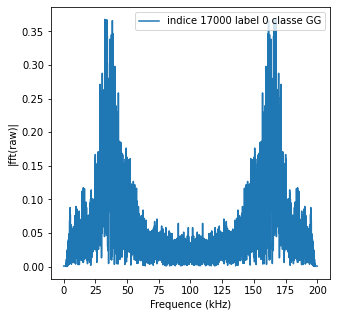
\includegraphics[width=\textwidth]{./images/17000fft.png}
  \end{subfigure}
  \begin{subfigure}[b]{0.3\textwidth}
    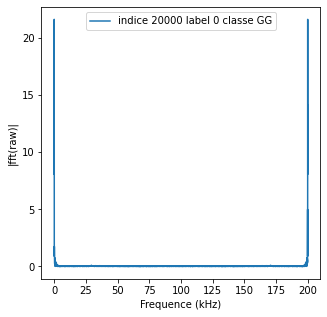
\includegraphics[width=\textwidth]{./images/20000fft.png}
  \end{subfigure}
  \begin{subfigure}[b]{0.3\textwidth}
    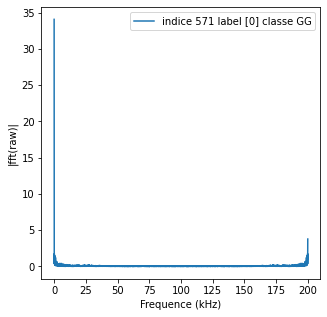
\includegraphics[width=\textwidth]{./images/571fft.png}
  \end{subfigure}
  \caption{Transformé de Fourier des signaux : (a) n°17000 et (b) n°20000 de la base d'apprentissage ; (c) n°571 de la base de test.%
\label{fig:tf}}
\end{figure}

Sur la figure \ref{fig:tf} on constate particuliérement sur le signal n° 17000

\hypertarget{Spectrogrammes}{%}
\subsection{Spectrogrammes}
\label{Spectrogrammes}}

Les Spectrogrammes sont simplement des transformé de fourier non pas sur l'ensemble de l'enregistrement mais a chaque échantillon, ainsi si l'échantillon est de 100 millisecondes par exemple le spectrogramme seras un enchainement de transformé de fourier toutes les 100 millisecondes.

On commence tout d'abord par observer leurs Spectrogrammes en 2D (a noter qu'ici pour éviter les phénoménes d'écrasement (les fréquences majoritaires pouvant écraser les autres) on utilise une échelle logarithmique):

\begin{figure}[!h]
  \centering
  \begin{subfigure}[b]{0.3\textwidth}
    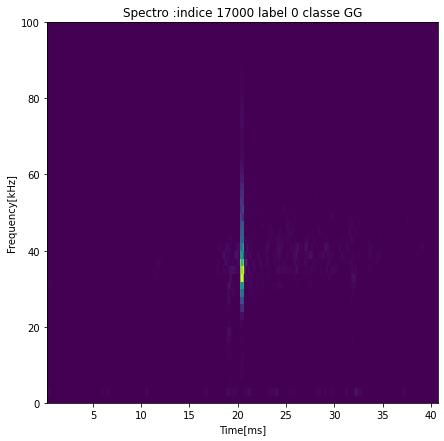
\includegraphics[width=\textwidth]{./images/indice17000Spectro2Dlabel0classeGGsansprocessingsanszoom.png}
  \end{subfigure}
  \begin{subfigure}[b]{0.3\textwidth}
    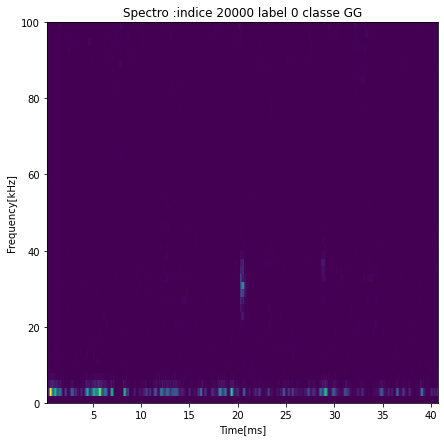
\includegraphics[width=\textwidth]{./images/indice20000Spectro2Dlabel9classeZCsansprocessingsanszoom.png}
  \end{subfigure}
  \begin{subfigure}[b]{0.3\textwidth}
    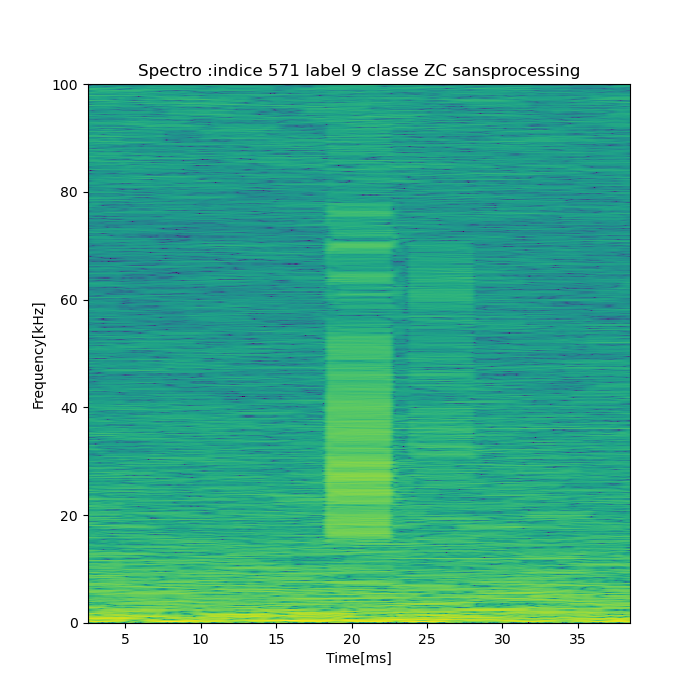
\includegraphics[width=\textwidth]{./images/indice571Spectro2Dlabel9classeZCsansprocessingsanszoom.png}
  \end{subfigure}
  \caption{Spectrogramme 2D des signaux : (a) n°17000 et (b) n°20000 de la base d'apprentissage ; (c) n°571 de la base de test.%
  \label{fig:spectros2D}}
\end{figure}

On constate tout d'abord  que leurs gamme de fréquence semble relativement variable d'un enregistrement à l'autre et que la visibilité des clics semble bien correlé à leur qualité ainsi sur le signal n° 17000 qui est le meilleur le clic est très clairement visible, sur le signal n° 571 qui est dégradé le clic est encore assez visible contrairement au signal n° 20000 qui est le plus dégradé dont le clic est très peux visible.

Puis on observe les Spectrogrammes 3D:

\begin{figure}[!h]
  \centering
  \begin{subfigure}[b]{0.3\textwidth}
    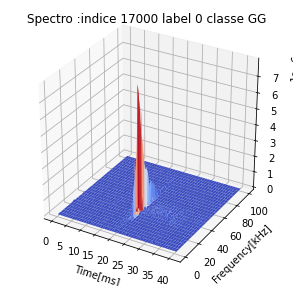
\includegraphics[width=\textwidth]{./images/indice17000Spectro3Dlabel0classeGGsansprocessingsanszoom.png}
  \end{subfigure}
  \begin{subfigure}[b]{0.3\textwidth}
    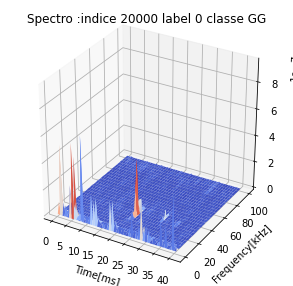
\includegraphics[width=\textwidth]{./images/indice20000Spectro3Dlabel9classeZCsansprocessingsanszoom.png}
  \end{subfigure}
  \begin{subfigure}[b]{0.3\textwidth}
    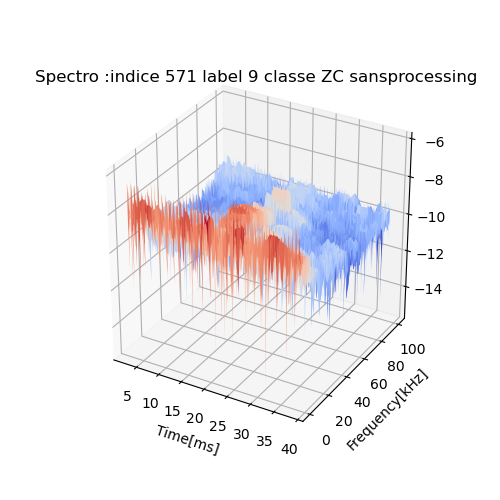
\includegraphics[width=\textwidth]{./images/indice571Spectro3Dlabel9classeZCsansprocessingsanszoom.png}
  \end{subfigure}
  \caption{Spectrogramme 3D des signaux : (a) n°17000 et (b) n°20000 de la base d'apprentissage ; (c) n°571 de la base de test.%
  \label{fig:spectros3D}}
\end{figure}

\hypertarget{Data-augmentation}
\subsection{Intérêt théorique}
\label{interets_theoriques}}

Basiquement la Data augmentation regroupe un ensemble de méthodes permettant d'augmenter "artificiellement" la taille de la base sur laquelle notre IA va apprendre. Ainsi en plus de nos exemples initiaux on viendra rajouter de nouveaux exemples qui seront des versions "modifiées" des exemples initiaux.

Pour cela selon la nature des données de cette base on va par exemple :
\begin{itemize}
\item Flouter les exemples s'il s'agit d'images
\item Effectuer une rotation sur les exemples
\item Modifier la luminosité dans le cas d'images
\end{itemize}

Dans notre cas vus que nos données sont des enregistrements audios on va plutôt :
\begin{itemize}
\item Rajouter du bruit sur les exemples
\item Déplacer le clic
\item Simuler une modification de la distance entre l'animal et le micro
\end{itemize}

L'intérêt le plus évident de cette opération est de simplement multiplier le nombre d'exemples disponibles afin d'éviter le surapprentissage mais elle peut avoir beaucoup plus d'utilité. En effet dans notre cas nous n'avons rencontré aucun probléme de surapprentissage mais nous avions besoin de l'utiliser pour une autre raison.
Effectivement nous avions remarqué que certains exemples avaient subis de fortes dégradations notament dues à du bruit ou bien à un fort décalage temporel du clic par exemple. Afin d'éviter que ces dégradations n'altérent le processus d'apprentissage de nos réseaux de neurones (le réseau pouvant par exemple assimiler une de ces dégradations a l'une des classes) plutôt que de supprimer ces dégradations il nous a paru plus pertinent de d'abord essayer de rajouter des exemples avec des dégradations similaires issuent d'exemples choisis aléatoirement parmis nos classes sur lesquelles ont aurait fait de la data augmentation. En effet ces dégradations pouvant être simplement dues a des problémes pendant l'enregistrement des clics (bateau navigant a proximité du micro ou encore d'autres animaux émettant divers bruits à proximité par exemple) il est plus que problable que les enregistrements qui seront soumis par la suite à notre classifieur contiennent également des dégradations qui ne devront pas entraver le bon fonctionnement de celui-ci.

\hypertarget{Rajout-de-bruit-blanc}
\subsection{Simulation de distance}
\label{Simulation-de-distance}}

Lors de la prise des enregistrements audios les animaux peuvent se situer plus ou moins loin du ou des micro, ce qui peux potentiellement influencer notre classifieur. En effet certaines especes plus fuyardes peuvent par exemple rester systématiquement plus éloignées du micro que les autres poussant le classifeur a assimiler une grande distance a une éspece en particulier.
Afin d'éviter ce biais nous avons décidé de rajouter la simulation de distance dans la data augmentation.
Le principe est simple on vas rajouter aléatoirement des signaux choisis dans des classes aléatoires a une distance aléatoire (on simule les effets de la distance sur le signal).

\hypertarget{Traitement-du-signal}{%}
\section{Traitement du signal}
\label{Traitement-du-signal}}

Comme nous avons pu le voir précedement il arrive que certains enregistrements aient subis d'importantes dégradations, si dans un premier temps nous avons fait de la data augmentation il pouvait y avoir certains enregistrements pour lesquels cela ne suffis pas. Parcequ'ils seraient trop dégradés ils empêcheraient l'identification de l'espece, cela peut être un bruit tellement important qu'il recouvrirait le clic par exemple. Ainsi nous avons quand même dû faire du traitement du signal. Ces traitements ne vont pas remplacer la data augmentation déjà effectué mais viendrons simplement en complément de celle ci

\hypertarget{Filtre-passe-haut}{%}
\subsection{Filtre passe haut}
\label{Filtre-passe-haut}}

Dans un premier temps pour résoudre les probléme vus précedement on  vas commencer par appliquer un filtre passe haut aux enregistrements. En effet les clics des différents animaux se situant dans une gamme de fréquence au dessus des 8 KHz on peux donc appliquer le filtre à l'enregistrement sans en altérer le clic.
Sur la réponse fréquencielle du filtre on peux observer
\begin{figure}[!h]
\centering
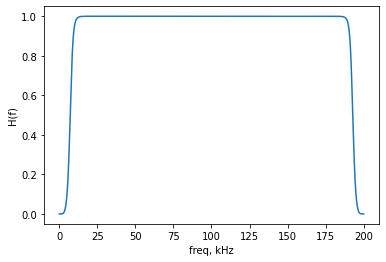
\includegraphics[width=\textwidth]{./images/reponseEnFrequencePH8kHz.png}
\caption{Réponse fréquencielle du passe haut à 8kHz%
\label{fig:reponseEnFrequencePH8kHz}}
\end{figure}
Sur la réponse fréquencielle du filtre \ref{fig:reponseEnFrequencePH8kHz} on peux observer qu'au niveau de la fréquence de coupure qui est de 8kHz on 
Ainsi en appliquant simplement ce filtre on constate par exemple que l'identification du clic pour le zoom qui était impossible sans le filtre (à gauche sur \ref{fig:20000zoomavecetsansfiltrage}) sur le signal n° 20000 deviens parfaitement possible avec (à droite sur \ref{fig:20000zoomavecetsansfiltrage}) :

\begin{figure}[!h]
\centering
  \begin{subfigure}[b]{0.45\textwidth}
    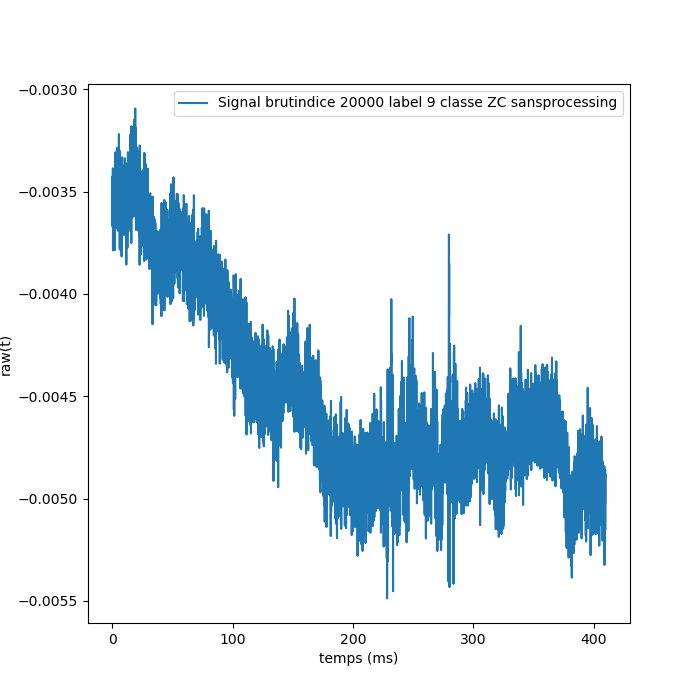
\includegraphics[width=\textwidth]{./images/indice20000Spectro1Dlabel9classeZCsansprocessingsanszoom.png}
  \end{subfigure}
  \begin{subfigure}[b]{0.45\textwidth}
    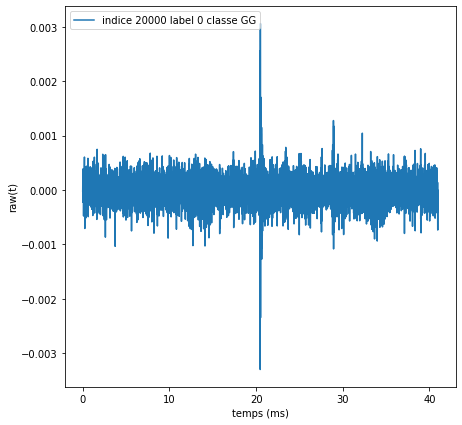
\includegraphics[width=\textwidth]{./images/indice20000Spectro1Dlabel9classeZCavecprocessingsanszoom.png}
  \end{subfigure}
  \caption{Spectrogramme 3D des signaux : (a) n°20000 de la base d'apprentissage zoomé et non filtré et (b) n°20000 de la base d'apprentissage zoomé et filtré%
\label{fig:20000zoomavecetsansfiltrage}}
\end{figure}

\hypertarget{Mise-a-l-echelle}{%}
\subsection{Mise à l'échelle}
\label{Mise-a-l-echelle}}

En analysant les signaux on a constaté de grandes différences aussi bien en terme d'intensité que de fréquences sur leurs clics, hors pour bien fonctionner le réseau de neurones convolutif a besoin de données à la même échelle. C'est pourquoi on vas devoir mettre à l'échelle nos signaux, autrement dit on vas normaliser automatiquement entre 1 et -1 l'ensemble de nos signaux.
Afin de réaliser celà on fais un choix pragmatique qui était de réperer le maximum puis diviser le signal par ce maximum
\comment a revoir

\hypertarget{Les-Pipelines}{%}
\section{Les Pipelines}
\label{Les-Pipelines}}

A l'image des pipelines utilisés pour transporter le gaz ou le pétrole, les pipelines en informatique servent à transporter un flux de données.
Flux de données sur lequel on va effectuer un certain nombre d'opérations, flux qui sera ensuite injecté directement dans le réseau de neurones.
Cette méthode présente plusieurs interets majeurs :
\begin{itemize}
\item Premièrement elle nous évite de stocker le résultat des opérations intermédiaires  faisant gagner beaucoup de mémoire
\item Deuxièmement elle nous permet d'optimiser grandement l'ensemble du processus de prétraitement des données.
\item Troisièmement ce procédé améliore grandement les performances de tensorflow
\end{itemize}

En pratique l'ensemble de nos fonctions étaient stockées dans un fichier python nommé cachalot helper, et à chaque essai on faisait passer notre flux de données par les fonctions désirées avant de l'injecter dans le réseau de neurones.


\hypertarget{Les-PDF}
\subsection{Génération des PDF}
\label{Guxe9nuxe9ration-des-PDF}}

Les bases de données contiennent un très grand nombre d'exemples (environ 90 000 au total que l'on peut visualiser sous 12 formes différentes soit potentiellement 1 080 000 images).
Afin de pouvoir exploiter les analyses faites précedement il a fallu créer un certain nombre d'outils afin de pouvoir aisement trier et manipuler les données.
Pour cela je me suis inspiré du systéme de pipeline que nous venons de voir, ainsi dans un premier temps l'ensemble des fonctions nécessaires à l'analyse étaient stockés dans le cachalot{\_}helper.

Dans un second temps j'ai créer dans un autre python une fonction paramètrable permettant tout d'abord de sélectionner ou un certain nombre de signaux dans un certain nombre de labels ou des signaux bien specifiques puis de générer (à l'aide du cachalot{\_}helper) avec et ou sans preprocessing (les traitements du signal) avec ou sans zoom :
\begin{itemize}
\item Des plots des signaux sélectionnés
\item Des spectrogrammes 2D des signaux sélectionnés
\item Des spectrogrammes 3D des signaux sélectionnés
\end{itemize}
Une fois générés ils sont enregistrés sous forme de png dont le nom correspond à leur description. Ce qui donne par exemple pour le spectrogramme 3D sans processing et sans zoom de l'enregistrement numéro 17 000 de la classe GG dont le label est 0 :
indice17000Spectro3Dlabel0classeGGsansprocessingsanszoom.png. A noter que les plots simples sont enregistrés sous spectro1D pour des raisons pratiques.

Dans un troisième temps j'ai créé un autre python également paramètrable permettant de sélectionner des png en fonction de leur label de leur type (spectrogramme 1D ou 2D ou 3D) et leurs options (avec ou sans zoom et avec ou sans processing). Puis ils sont stockés dans un ou plusieurs fichiers tex en fonction de leur nombre.

Dans un quatrième temps j'ai créé un autre python encore une fois paramètrable qui va récupérer les fichiers tex précedement créés. Puis il va les réunir dans un seul fichier tex. Fichier tex qui va automatiquement s'executer pour générer un fichier pdf. Fichier pdf qui contient l'ensemble des courbes qui étaient stockées dans les fichiers tex. Ce fichier pdf sera alors enregistré son nom correspondant à ce qu'il contient. Ainsi un fichier contenant les spectrogrammes 2D du label 6 sans processing et zoomer sera nommé: Spectro2Dlabel6sansprocessingaveczoom.pdf

Et enfin un programme principal nommé apdfmaker également paramètrable chargé de faire tourner l'ensemble des programmes vus précedement. Dans le but de générer directement des fichiers pdf contenant ce que l'on désire. A noter que celui ci ne se contente pas de générer un pdf à la fois mais peut au contraire en générer une multitude à chaque run. Ainsi si l'on veut par exemple qu'il génére toutes les représentations graphiques possibles (soit 1 080 000 images) de tous les enregistrements puis qu'il les stocke dans des pdf le plus détaillés possibles c'est parfaitement possible.

\hypertarget{Ruxe9sultats-de-l-analyse-des-PDF}{%}
\subsection{Résultats de l'analyse des PDF}
\label{Ruxe9sultats-de-l-analyse-des-PDF}}
